\documentclass[10pt,a4paper]{article}
\usepackage{fontspec,polyglossia}\setmainlanguage{russian}\setmainfont{Times New Roman}
\usepackage{amsmath,amssymb,booktabs,tabularx,graphicx}\usepackage[margin=17mm]{geometry}
\usepackage[hidelinks]{hyperref}\usepackage{titlesec}\titleformat{\section}{\large\bfseries}{}{0pt}{}
\titlespacing*{\section}{0pt}{8pt}{4pt}\setlength{\parindent}{0pt}\setlength{\parskip}{4pt}\setlength{\emergencystretch}{3em}
\begin{document}
{\Large\bfseries MG обнаруживает упрощение управляющих сигналов обучаемой политики Walker2d}\par\medskip

Итоговый отчёт по завершённой серии экспериментов

\section*{Основной результат и сильные стороны метода}

\textbf{MG по одному скалярному логу устойчиво реагирует на упрощение управляющих команд при дообучении политики.} При умеренной регуляризации оценка нормы действия уменьшается примерно на 20\% и 40\%; знак подтверждён на всех пяти проверочных сидах. Снижение независимо сопровождается более плавными командами и меньшей ошибкой повторения состояния. При чрезмерной регуляризации MG перестаёт следовать улучшению плавности: его рост показывает дополнительное изменение структуры сигнала в режиме ухудшения ходьбы.

В этом опыте наиболее сильны три свойства MG: \textbf{воспроизводимость на разных сидах и скалярных логах; чувствительность к умеренному вмешательству; информация сверх величины соседних приращений}. Метод применён к поведению обучаемой нейросетевой политики в задаче управления. Практическая ценность здесь --- возможность анализировать изменения по компактному логу, не сохраняя полную траекторию состояния для самого расчёта MG.

\section*{Что обучается и зачем}

В симуляторе Walker2d двуногий агент должен продолжать движение вперёд, сохраняя устойчивость. Нейросетевая политика получает 17 наблюдений и выдаёт шесть команд суставам. PPO дообучает уже ходящего агента. Цель вмешательства --- получить более плавное управление при сохранении награды исходной задачи. Это мотивирует постановку для контроля качества управляющих политик; износ приводов и перенос на реального робота здесь не измерялись.

К функции потерь PPO добавлен штраф за изменение среднего действия на соседних состояниях:

\[
L=L_{\mathrm{PPO}}+\frac{\lambda}{6}\,\mathbb{E}_{(s_t,s_{t+1})}
\|\bar a_\theta(s_{t+1})-\bar a_\theta(s_t)\|_2^2,
\qquad \bar a_\theta(s)=\operatorname{clip}(\mu_\theta(s),-1,1).
\]

$\theta$ --- параметры политики, $s_t$ --- состояние, $\mu_\theta$ --- среднее её распределения действий. Пары берутся из собранных при обучении переходов без пересечения границ эпизодов; число случайных пар равно размеру минибатча. Штраф действует на среднюю команду, а не на исследовательский шум. Награда среды остаётся прежней.

\textbf{Обучение и измерение разделены:} на выбранном этапе веса политики фиксируются, агент выполняет тестовые эпизоды, и MG рассчитывается по последовательности его команд. Сравнение чекпоинтов показывает, как меняется поведение по мере обучения; MG здесь не рассчитывается по весам или training loss.

\section*{Воспроизводимая постановка}

\begin{center}\small
\begin{tabularx}{\linewidth}{l>{\raggedright\arraybackslash}X}
\toprule
Элемент & Зафиксированная настройка \\
\midrule
Сравнение & $\lambda=0,0.25,1,4$; ноль --- PPO без добавленного штрафа \\
Повторения & Пять сидов 231--235 из общего исходного checkpoint: 20 обучений \\
Архитектура & Отдельные актор и критик, по два слоя 64--64 с Tanh \\
Бюджет & 1048576 переходов на обучение; 8 сред, rollout 512, batch 256, 5 эпох \\
PPO & LR от $3\cdot10^{-5}$ до $3\cdot10^{-6}$; clip 0.1, target KL 0.01 \\
Остальные параметры & $\gamma=0.99$, GAE 0.95, entropy 0, value 0.5, gradient clipping 0.5 \\
Нормализация & Статистика наблюдений и наград заморожена из исходного checkpoint \\
Финальные тесты & 10 общих reset 62001--62010 на вариант: 200 эпизодов \\
Запись & Детерминированные действия; 512 шагов разогрева и 4096 анализа; шаг 0.008 с \\
MG & Окно 2048, задержка 8, $E=20$, 20 соседей, Theiler 312; проверка $E=40$ \\
\bottomrule\end{tabularx}\end{center}

Основной скаляр --- $x_t=\|a_t\|_2$, где $a_t\in\mathbb R^6$ --- исполненные команды. Дополнительные логи: $\|a_t-a_{t-1}\|_2$ и среднее шести команд. MG --- медиана окон с концами 2048, 3072, 4096; dither $10^{-9}$, seed оценщика 123. Настройки перенесены из предыдущего этапа, без подбора по проверочным результатам. Пилотный сид 230 в итоговые числа не включён.

Успех эпизода: полная запись без падения, средняя скорость не ниже 0.5. Для анализа также нужны стандартное отклонение угла правого колена не ниже 0.05 и восемь пиков (расстояние 20, prominence 0.15). Падения не превращаются в нулевой MG; они остаются в показателях качества. Награда делится на фиксированные 4096 шагов, отсутствующий после падения остаток даёт нулевой вклад. Единица повторения --- обучающий сид, а не отдельное окно.

\newpage

\section*{Устойчивый сигнал при сохранении качества управления}

В таблице MG --- медиана по пяти сидам: внутри сида сначала берётся медиана отношений к контролю на общих допустимых reset. Награда --- отношение средних по всем 50 эпизодам группы, включая падения. Число пригодных пар с контролем: 48, 47, 45 и 24 соответственно.

\begin{center}\small
\begin{tabularx}{\linewidth}{l>{\raggedright\arraybackslash}X>{\raggedright\arraybackslash}X>{\raggedright\arraybackslash}X>{\raggedright\arraybackslash}X}
\toprule
Штраф $\lambda$ & Успешные эпизоды & Награда / контроль & MG / контроль & Сидов со снижением MG \\
\midrule
0 & 48/50 & 1.000 & 1.000 & --- \\
0.25 & 49/50 & 1.020 & \textbf{0.801} & \textbf{5/5} \\
1 & 47/50 & 0.978 & \textbf{0.604} & \textbf{5/5} \\
4 & 25/50 & 0.681 & 1.114 & 1/5 \\
\bottomrule\end{tabularx}\end{center}

\textbf{Результат не держится на одном удачном запуске.} Для слабого штрафа отношения MG по отдельным сидам лежат в диапазоне 0.582--0.845, для умеренного --- 0.509--0.781. В обоих случаях снижение воспроизводится на каждом сиде. На двух дополнительных скалярах знак также сохраняется на 5/5 сидов: при $\lambda=0.25$ отношения равны 0.662 и 0.742, при $\lambda=1$ --- 0.601 и 0.651. Эти проверки связаны между собой и не считаются дополнительными независимыми обучениями.

\begin{center}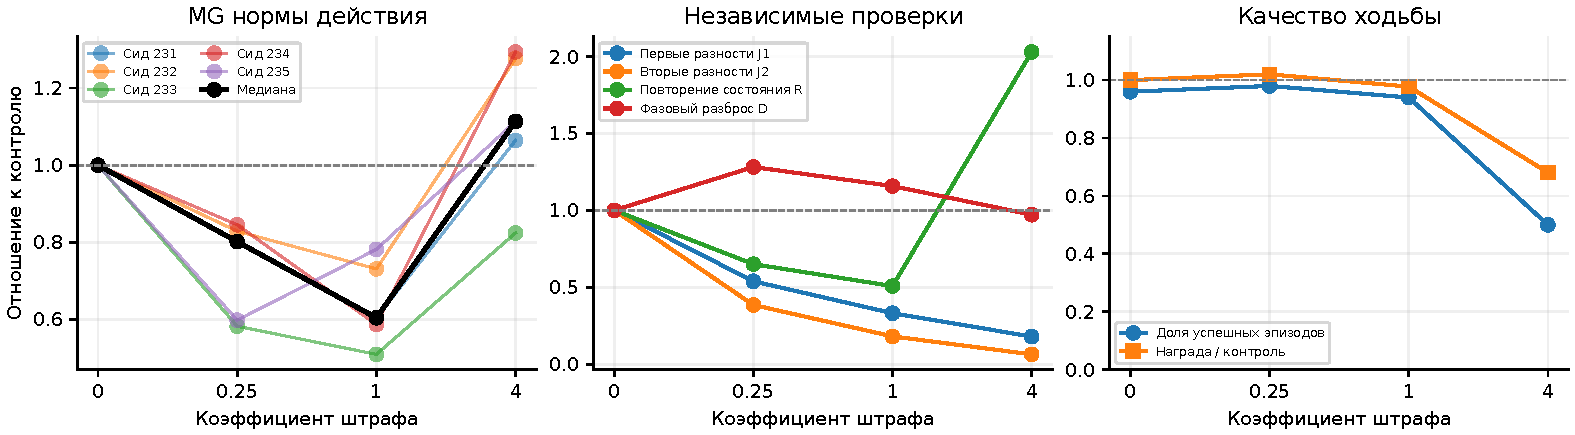
\includegraphics[width=\linewidth,height=.32\textheight,keepaspectratio]{final_evidence.pdf}\end{center}

\section*{Независимое подтверждение изменения поведения}

Плавность оценивалась по средним квадратам первых и вторых разностей шестимерной команды; $T=4096$ --- длина записи:

\[
J_1=\frac{1}{6(T-1)}\sum_{t=1}^{T-1}\|a_t-a_{t-1}\|_2^2,\qquad
J_2=\frac{1}{6(T-2)}\sum_{t=2}^{T-1}\|a_t-2a_{t-1}+a_{t-2}\|_2^2.
\]

При $\lambda=0.25$ отношения $J_1,J_2$ к контролю равны 0.539 и 0.385; при $\lambda=1$ --- 0.331 и 0.181. Полносостоянийная ошибка повторения $R$ уменьшается до 0.650 и 0.508. Она равна минимуму среднего квадрата расстояний между состояниями через лаг 20--250, делённого на удвоенную дисперсию состояния. Для неё используются восемь координат положения без горизонтального переноса и девять скоростей, поделённых на 5. Эти измерения вычисляются независимо от MG; $J_1$ близок к самому обучающему штрафу.

Таким образом, снижение MG сопровождается наблюдаемым изменением поведения: команды менее резкие, состояние лучше повторяется через фиксированный лаг. Это содержательная проверка скалярного сигнала в системе с обучением. Другой критерий, разброс состояния в моменты пиков правого колена, не уменьшается устойчиво; поэтому подтверждение относится к указанным свойствам, а не ко всем аспектам движения.

\section*{MG не сводится к показателю плавности}

При $\lambda=4$ первые и вторые разности команд продолжают уменьшаться: отношения $J_1=0.180$, $J_2=0.064$. Тем не менее качество ходьбы резко хуже, а MG нормы действия растёт относительно контроля на 4/5 сидов. На 24 общих пригодных тройках эпизодов вариантов 0, 1 и 4 отношение MG сильного штрафа к умеренному равно \textbf{1.704; рост на 5/5 сидов}. Нормированная энергия приращений того же скаляра при этом уменьшается до 0.770.

Это показывает полезную дополнительную чувствительность MG: более плавный лог не обязательно получает меньшую оценку. Проверка всей кривой на 23 наборах reset, пригодных во всех четырёх вариантах, сохраняет результат. Сравнение условно на успешных эпизодах и не является проверкой раннего предупреждения о падении.

\newpage

\section*{Чувствительность по ходу обучения и сравнение с простыми метриками}

На пяти фиксированных этапах обучения всех 20 политик дополнительно проверен reset 62001. При $\lambda=0.25$ медианное отношение MG меняется как 1.000, 0.811, 0.808, 0.747, 0.745 после 0, 262144, 524288, 786432 и 1048576 переходов; число пригодных пар --- 5, 5, 5, 4, 5. \textbf{Сигнал появляется уже на первом проверенном промежуточном этапе}, что поддерживает использование MG для периодического анализа поведения обучаемой политики. Это не доказательство монотонности: для других коэффициентов кривые немонотонны, а состав выживших пар меняется.

Все скалярные конкуренты получали те же записи и окна. Спектральная энтропия $H$ измеряет концентрацию мощности по частотам; $Q$ --- средний квадрат соседнего приращения, нормированный на удвоенную дисперсию; $R_x$ --- аналогично нормированная ошибка повторения скаляра при лучшем лаге 20--250. В ячейке ниже: отношение к контролю и число сидов со снижением.

\begin{center}\small
\begin{tabularx}{\linewidth}{l>{\raggedright\arraybackslash}X>{\raggedright\arraybackslash}X}
\toprule
Показатель & Слабый штраф, $\lambda=0.25$ & Умеренный штраф, $\lambda=1$ \\
\midrule
\textbf{MG} & \textbf{0.801; 5/5} & \textbf{0.604; 5/5} \\
Спектральная энтропия $H$ & 0.996; 4/5 & 0.958; 3/5 \\
Ошибка повторения $R_x$ & 0.799; 4/5 & 0.790; 5/5 \\
Нормированные приращения $Q$ & 0.809; 4/5 & 0.598; 5/5 \\
\bottomrule\end{tabularx}\end{center}

\textbf{Наблюдаемое преимущество MG --- устойчивость знака при умеренном вмешательстве.} Для основного скаляра энтропия меняется слабо и менее согласованно по сидам; при слабом штрафе каждый простой конкурент даёт нужный знак на 4/5, а MG --- на 5/5. При пяти сидах это описательный результат, а не установленное статистическое превосходство. Величины измеряют разные свойства: больший процент изменения сам по себе не означает лучшую диагностику.

Ошибка повторения остаётся сильным конкурентом: на двух дополнительных логах она, как и MG, снижается на 5/5 сидов при обоих умеренных штрафах. При сильном штрафе она растёт относительно контроля на всех пяти сидах для всех трёх логов; MG такой универсальности относительно контроля не показывает. При прямом сравнении 4 с 1 оба метода растут на 5/5 для каждого лога. Следовательно, MG даёт полезную характеристику структуры сигнала, но уникальная диагностическая возможность по сравнению с $R_x$ здесь не установлена.

\section*{Компактное наблюдение и измеренная стоимость}

Для MG достаточно сохранять один вычисляемый из команд скаляр; полное состояние, веса политики и производные модели ему не передаются. Полное состояние использовано в эксперименте для независимой проверки. Это достоинство по требованиям к наблюдению относительно полносостоянийного анализа; простые скалярные конкуренты обладают тем же свойством.

Замер: одинаковое окно из памяти, CPU, один поток, прогрев и семь повторов в перемешанном порядке; без чтения и сбора данных. Медианы:

\begin{center}\small
\begin{tabularx}{\linewidth}{l>{\raggedright\arraybackslash}X}
\toprule
Расчёт & Время на окно \\
\midrule
MG, $E=20$ & \textbf{0.369 с} \\
MG с дополнительной проверкой $E=40$ & 0.774 с \\
Скалярная ошибка повторения & 3.782 мс \\
Спектральная энтропия & 0.103 мс \\
Нормированные приращения & 0.048 мс \\
\bottomrule\end{tabularx}\end{center}

MG занимает меньше секунды на окно в отдельном замере: это аргумент для периодического анализа сохранённых логов, но не проверка реального времени или нагрузки на обучение. Ошибка повторения здесь в 98 раз быстрее. Преимущество MG по скорости не установлено; сравнение со спектрами Ляпунова не проводилось.

\section*{Итоговая формулировка для статьи}

\textbf{В задаче управления Walker2d оценка MG по одному агрегированному логу команд устойчиво обнаруживает изменения, сопровождающие упрощение управляющего сигнала при дообучении политики. Эффект воспроизводится на пяти сидах и трёх скалярных наблюдаемых и согласуется со снижением резкости команд и ошибки повторения состояния. При чрезмерной регуляризации MG может возрастать, несмотря на дальнейшее сглаживание команд, отражая свойства временной структуры сверх локальной плавности.}

Граница вывода: вмешательство задано явно, исходный checkpoint общий, тестовые reset использовались ранее. Число активных компонент неизвестно, предпосылки точной размерностной интерпретации не подтверждены, фазовый разброс состояния не улучшился. Результат поддерживает MG как анализатор упрощения выбранного лога; не устанавливает уменьшение размерности всей системы, превосходство над всеми простыми метриками или прогнозирование отказов. Данные и воспроизведение: README.md. Итоговый отчёт: 1 октября 2026 года.
\end{document}